\chapter{Git, worktrees, and isolated execution}

\section{Engineering principles}

A linked worktree gives each task its own checkout and index while sharing portions of repository metadata. It is useful for concurrency but is not a filesystem, process or network sandbox. A malicious or compromised process with sufficient OS access may inspect or alter other worktrees or shared repository state.\src{G1}

\section{Implementation approach}

Create a branch per task from a reviewed base SHA using git worktree add. Give each worker a distinct directory and record the branch. Inspect status and diff before commit. Integrate branches only after independent checks and human review. Remove completed worktrees with git worktree remove after preserving required evidence; do not force removal of dirty work. Use separate clones or stronger isolation for mutually untrusted workers.

\section{Verification and limitations}

Test that simultaneous tasks do not modify the same files and that shared metadata cannot be accessed by untrusted workers in the production isolation design. A worktree alone cannot satisfy the second requirement.

Figure~\ref{fig:d16} illustrates the conceptual flow from Base commit to Reviewed merge. The edges describe the proposed integration or control relationship, not undocumented internal calls.

\begin{figure}[htbp]\centering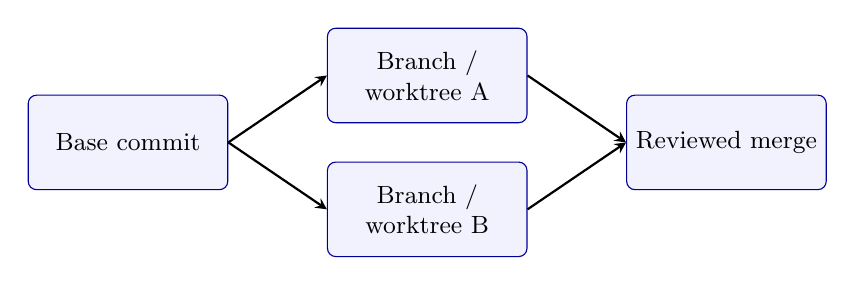
\begin{tikzpicture}[nodebox/.style={draw=blue!60!black,fill=blue!5,rounded corners=3pt,minimum height=12mm,text width=23mm,align=center,font=\small},>=stealth]
\node[nodebox] (n0) at (0.00,0.00) {Base commit};
\node[nodebox] (n1) at (3.80,0.85) {Branch / worktree A};
\node[nodebox] (n2) at (3.80,-0.85) {Branch / worktree B};
\node[nodebox] (n3) at (7.60,0.00) {Reviewed merge};
\draw[->,thick] (n0.east) -- (n1.west);
\draw[->,thick] (n0.east) -- (n2.west);
\draw[->,thick] (n1.east) -- (n3.west);
\draw[->,thick] (n2.east) -- (n3.west);
\end{tikzpicture}
\caption{Git worktree isolation (conceptual view).}\label{fig:d16}\end{figure}

\section{Chapter conclusion}

Apply the stated verification criteria before expanding the scope of this workflow. Record deviations, evidence and unresolved risks in the task record.
